\subsection{Preregistered objective known-world confirmatory result}
\label{sec:objective-confirmatory}

The historical Q1--Q4 diagnostic uses internally proposed cases and therefore cannot by itself establish an external transfer-validity construct. We consequently registered a separate objective lane in which the correct transfer decision is obtained by executing a family-specific target-world verifier rather than by an annotator or by the generator's perturbation identity. The primary v1 scope was frozen before confirmatory outcome access to four heterogeneous exact-verifier families: mapped directed-flow feasibility, Horn-style logical entailment, dimensional/unit transformations and finite deterministic state-transition systems. The first development instrument failed the preregistered coordinate-ablated-twin circularity attack and was preserved as negative history rather than promoted. A redesigned development instrument passed the registered semantic-difficulty and circularity checks; its paired binary-Brier variance gave a required decidable sample of 431 for the registered 0.05 MDE. Before generating confirmatory outcomes we therefore froze seed \texttt{2026081202}, 16 instances per base cell and $n=576$ total cases. The freeze was merged to the public repository before that seed was executed.

The fresh confirmatory packet contained 256 verifier-licensed transfers, 256 verifier-rejected transfers and 64 \texttt{CANNOT\_CHECK} cases. A lexical/Jaccard control remained near chance on the 512 decidable cases (accuracy $0.496$). More importantly, the strongest deterministic structural control in this lane was not lexical: a derived-effect or ``mechanism-only'' rule already reached exact three-way accuracy $0.875$, accepted every valid transfer and rejected every registered semantic-near-miss case, but still licensed $25\%$ of all verifier-invalid transfers because mechanism preservation alone did not enforce every applicability coordinate. A relation/invariant-only control reached exact accuracy $0.819$ with invalid-transfer false-accept $0.375$. The full applicability contract---QoI, boundary, mapping, relations, source preconditions/invariants and independently derived target effect---matched all 576 exact-verifier decisions, retaining every valid transfer, falsely licensing no invalid transfer and abstaining on every verifier-unknown case.

The preregistered primary residual is therefore the full contract relative to the mechanism-only control rather than the much easier lexical comparison. On the 512 decidable cases, the paired binary-Brier reduction was $0.120$ with an item-bootstrap 95\% interval $[0.0938,0.1481]$ from 20,000 resamples, exceeding the registered 0.05 material-effect threshold (Figure~\ref{fig:objective-results}). The full-minus-mechanism exact-accuracy residual was positive in each of the four primary families.

\begin{figure}[t]
\centering
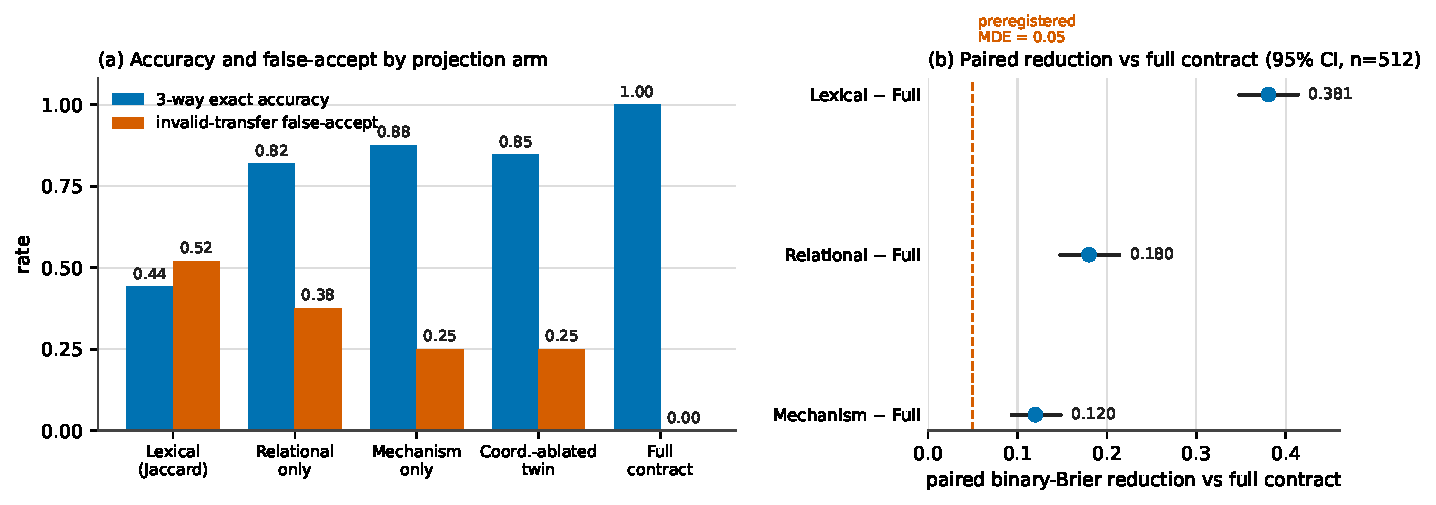
\includegraphics[width=\textwidth]{figures/objective_results.pdf}
\caption{Preregistered objective known-world confirmatory result (four families, $n=576$; $512$ decidable cases). \textbf{(a)}~Three-way exact accuracy and invalid-transfer false-accept rate for each projection arm, ordered by increasing applicability structure. The mechanism-only control already reaches $0.875$ exact accuracy yet still licenses $25\%$ of verifier-invalid transfers; only the full applicability contract attains exact accuracy $1.0$ with zero invalid false-accepts. \textbf{(b)}~Paired binary-Brier reduction of each control relative to the full contract with item-bootstrap $95\%$ confidence intervals (20{,}000 resamples); every reduction exceeds the preregistered $0.05$ material-effect threshold (dashed). Values are read directly from the committed frozen confirmatory evidence; the figure visualizes the primary four-family outcome only and does not use the pending six-family robustness extension. Because the full arm computes its coordinates from machine-readable target-world facts, the result establishes \emph{which} applicability coordinates a fail-closed gate must enforce, not that a system recovers them from unstructured prose.}
\label{fig:objective-results}
\end{figure} Four family clusters are nevertheless insufficient for a broad cross-domain law: the two-sided sign-test value for four positive family signs is $p=0.125$. A six-family robustness extension was named and frozen as a separate future coordinate before the primary outcomes; it is required before we claim broad family generalization.

This result is deliberately narrower than a model-level transfer claim. Candidate inputs in the objective lane expose machine-readable target-world facts from which the deterministic witness coordinates can be computed. The experiment therefore establishes that, in this generated exact-verifier scope, explicit applicability information resolves transfer decisions that remain ambiguous under relation-only and mechanism-only projections. It does not show that a language model can recover the witness from raw scientific prose, that a frontier direct-judgement model is inferior, that the same effect holds in natural scientific domains, or that witness gating improves end-to-end research outcomes. Strong semantic/LLM comparators, the disjoint downstream-routing study and independent natural-domain judgement remain separate evidence coordinates.

All four confirmatory packets are byte-reproducible from the committed generator, frozen seed and canonical JSONL serialization. Their expected SHA-256 identities, the paired inference, family analysis, anti-degeneracy audit and exact claim boundary are frozen in the committed confirmatory evidence packet.

\subsection{Preliminary external-model applicability-gate comparator}
\label{sec:llm-comparator}

The confirmatory lane above isolates \emph{which} applicability coordinates decide transfer, but it computes those coordinates from machine-readable target facts rather than asking a language model to apply them. We therefore ran a separate, independently frozen comparator that closes exactly this gap: it drives one fixed frontier model through the fail-closed applicability contract and measures whether the \emph{obligation structure}---not extra reasoning tokens---reduces invalid-transfer false-accepts. The design (three conditions, primary metric, hypothesis direction and stopping rule) was frozen before any model output was scored; a fresh benchmark seed (\texttt{20260812}) and $n\approx504$ exact-verifier tasks ($\geq$ the registered $n\approx431$ decidable target) were used, with the same three-way label space in every arm. The three conditions differ only in the instruction: a plain \textsc{Direct} judgement, a compute-matched \textsc{Free-CoT} control (``think step by step''), and the \textsc{Orion} gate (check each named applicability obligation; accept only if all load-bearing obligations are satisfied; reject on any violation; abstain if unverifiable).

\begin{figure}[t]
\centering
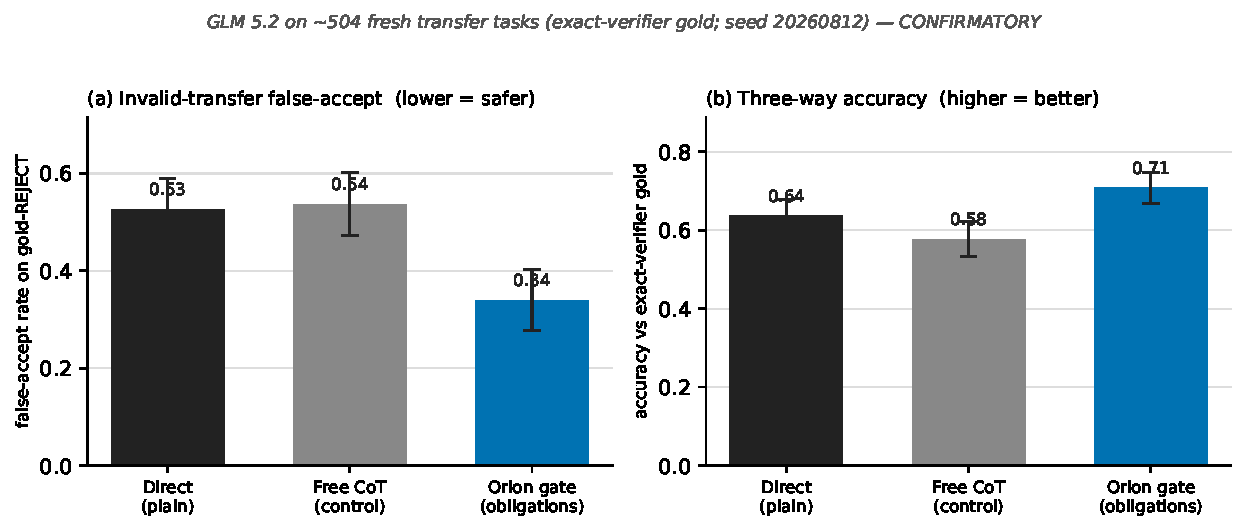
\includegraphics[width=\textwidth]{figures/llm_comparator.pdf}
\caption{Preliminary external-model applicability-gate comparator (one fixed frontier model; $n\approx504$ fresh exact-verifier tasks; bootstrap $95\%$ CIs, 20{,}000 resamples). \textbf{(a)}~Driving the model through the fail-closed applicability gate cuts the invalid-transfer false-accept rate from $0.527\,[0.460,0.589]$ (Direct) to $0.339\,[0.277,0.402]$ (gate); the two intervals do not overlap. The compute-matched Free-CoT control ($0.536\,[0.473,0.603]$) is statistically indistinguishable from Direct, so the reduction is attributable to the obligation \emph{structure}, not to additional reasoning. \textbf{(b)}~Three-way accuracy against exact-verifier gold rises in step ($0.637\!\to\!0.708$). This is a system/method effect (a structured-inference scaffold), not a claim that the model reasons better; on the hardest semantic near-miss decoys the gate does not beat Direct, a real and reported weakness.}
\label{fig:llm-comparator}
\end{figure}

Figure~\ref{fig:llm-comparator} shows the gate roughly halving the odds of licensing a verifier-invalid transfer while the compute-matched control moves nothing, which is the isolation the design was built to obtain: fail-closed applicability obligations, not more thinking, carry the reduction. We report this as a \emph{preliminary} comparator, deliberately outside the frozen four-family confirmatory packet governance above and subject to the same broadening the primary lane requires: it is one model, one seed and one benchmark family-set, it measures a scaffold rather than a smarter model, and it does not help on the trickiest semantic near-misses. A cross-model, cross-seed replication with the six-family sign test is the named next coordinate before any broad external-model claim.
